% Options for packages loaded elsewhere
\PassOptionsToPackage{unicode}{hyperref}
\PassOptionsToPackage{hyphens}{url}
%
\documentclass[
  a4paper,
]{book}
\usepackage{amsmath,amssymb}
\usepackage{iftex}
\ifPDFTeX
  \usepackage[T1]{fontenc}
  \usepackage[utf8]{inputenc}
  \usepackage{textcomp} % provide euro and other symbols
\else % if luatex or xetex
  \usepackage{unicode-math} % this also loads fontspec
  \defaultfontfeatures{Scale=MatchLowercase}
  \defaultfontfeatures[\rmfamily]{Ligatures=TeX,Scale=1}
\fi
\usepackage{lmodern}
\ifPDFTeX\else
  % xetex/luatex font selection
\fi
% Use upquote if available, for straight quotes in verbatim environments
\IfFileExists{upquote.sty}{\usepackage{upquote}}{}
\IfFileExists{microtype.sty}{% use microtype if available
  \usepackage[]{microtype}
  \UseMicrotypeSet[protrusion]{basicmath} % disable protrusion for tt fonts
}{}
\usepackage{xcolor}
\usepackage[left=2cm, right=1cm, top=2cm, bottom=2cm, twoside=false]{geometry}
\usepackage{longtable,booktabs,array}
\usepackage{calc} % for calculating minipage widths
% Correct order of tables after \paragraph or \subparagraph
\usepackage{etoolbox}
\makeatletter
\patchcmd\longtable{\par}{\if@noskipsec\mbox{}\fi\par}{}{}
\makeatother
% Allow footnotes in longtable head/foot
\IfFileExists{footnotehyper.sty}{\usepackage{footnotehyper}}{\usepackage{footnote}}
\makesavenoteenv{longtable}
\usepackage{graphicx}
\makeatletter
\def\maxwidth{\ifdim\Gin@nat@width>\linewidth\linewidth\else\Gin@nat@width\fi}
\def\maxheight{\ifdim\Gin@nat@height>\textheight\textheight\else\Gin@nat@height\fi}
\makeatother
% Scale images if necessary, so that they will not overflow the page
% margins by default, and it is still possible to overwrite the defaults
% using explicit options in \includegraphics[width, height, ...]{}
\setkeys{Gin}{width=\maxwidth,height=\maxheight,keepaspectratio}
% Set default figure placement to htbp
\makeatletter
\def\fps@figure{htbp}
\makeatother
\ifLuaTeX
  \usepackage{luacolor}
  \usepackage[soul]{lua-ul}
\else
  \usepackage{soul}
\fi
\setlength{\emergencystretch}{3em} % prevent overfull lines
\providecommand{\tightlist}{%
  \setlength{\itemsep}{0pt}\setlength{\parskip}{0pt}}
\setcounter{secnumdepth}{5}
% definitions for citeproc citations
\NewDocumentCommand\citeproctext{}{}
\NewDocumentCommand\citeproc{mm}{%
  \begingroup\def\citeproctext{#2}\cite{#1}\endgroup}
% avoid brackets around text for \cite:
\makeatletter
 \def\@biblabel#1{}
 \def\@cite#1#2{{#1\if@tempswa , #2\fi}}
\makeatother
\newlength{\cslhangindent}
\setlength{\cslhangindent}{1.5em}
\newlength{\csllabelwidth}
\setlength{\csllabelwidth}{3em}
\newlength{\cslentryspacing}
\setlength{\cslentryspacing}{0em}
\usepackage{enumitem}
\newlist{CSLReferences}{itemize}{1}
\setlist[CSLReferences]{label={},
  leftmargin=\cslhangindent,
  itemindent=-1\cslhangindent,
  parsep=\parskip,
  itemsep=\cslentryspacing}
\usepackage{calc}
\newcommand{\CSLBlock}[1]{#1\hfill\break}
\newcommand{\CSLLeftMargin}[1]{\parbox[t]{\csllabelwidth}{#1}}
\newcommand{\CSLRightInline}[1]{\parbox[t]{\linewidth - \csllabelwidth}{#1}\break}
\newcommand{\CSLIndent}[1]{\hspace{\cslhangindent}#1}
\ifLuaTeX
\usepackage[bidi=basic]{babel}
\else
\usepackage[bidi=default]{babel}
\fi
\babelprovide[main,import]{russian}
% get rid of language-specific shorthands (see #6817):
\let\LanguageShortHands\languageshorthands
\def\languageshorthands#1{}
\setmainfont{Georgia}
\setmonofont{Courier New}
\usepackage[fontsize=14pt]{scrextend}
\usepackage{indentfirst}
\setlength\parindent{12.7mm}
\pagestyle{plain}
\ifLuaTeX
  \usepackage{selnolig}  % disable illegal ligatures
\fi
\IfFileExists{bookmark.sty}{\usepackage{bookmark}}{\usepackage{hyperref}}
\IfFileExists{xurl.sty}{\usepackage{xurl}}{} % add URL line breaks if available
\urlstyle{same}
\hypersetup{
  pdftitle={Использование Markdown, RMarkdown и bookdown для подготовки научных отчетов и дипломных работ},
  pdfauthor={Н.О. Стрелков, В.В. Крутских},
  pdflang={ru},
  hidelinks,
  pdfcreator={LaTeX via pandoc}}

\title{Использование Markdown, RMarkdown и bookdown для подготовки научных отчетов и дипломных работ}
\author{Н.О. Стрелков, В.В. Крутских}
\date{2023-10-02}

\usepackage{amsthm}
\newtheorem{theorem}{Theorem}[chapter]
\newtheorem{lemma}{Lemma}[chapter]
\newtheorem{corollary}{Corollary}[chapter]
\newtheorem{proposition}{Proposition}[chapter]
\newtheorem{conjecture}{Conjecture}[chapter]
\theoremstyle{definition}
\newtheorem{definition}{Definition}[chapter]
\theoremstyle{definition}
\newtheorem{example}{Листинг}[chapter]
\theoremstyle{definition}
\newtheorem{exercise}{Exercise}[chapter]
\theoremstyle{definition}
\newtheorem{hypothesis}{Hypothesis}[chapter]
\theoremstyle{remark}
\newtheorem*{remark}{Remark}
\newtheorem*{solution}{Solution}
\begin{document}
\maketitle

\stepcounter{page}

\renewcommand*\contentsname{Содержание}
{
\setcounter{tocdepth}{4}
\tableofcontents
}
\chapter*{Аннотация}\label{index}
\addcontentsline{toc}{chapter}{Аннотация}

В настоящей работе рассматривается использование языка разметки Markdown для написания отчетов и дипломных работ. Используется расширение языка RMarkdown с дополнением bookdown. Демонстрируется применимость bookdown для оформления научных работ. Этот документ может быть использован как шаблон для подготовки текста работы.

\chapter*{Введение}\label{intro}
\addcontentsline{toc}{chapter}{Введение}

В настоящее время для написания дипломов, отчетов и научных работ широко используется Microsoft Word (далее MS Word). Следует отметить, что MS Word имеет следующие существенные недостатки:

\begin{itemize}
\tightlist
\item
  форматы doc и docx - бинарные (не текстовые), поэтому сложно сравнивать разные версии документа между собой и искать текст;
\item
  сложно организовать совместную работу;
\item
  сложно автоматизировать нумерацию разделов, рисунков, таблиц, формул, сносок, списка литературы, списка используемых сокращений, иллюстраций, алфавитных указателей в больших документах (книги, дипломы, диссертации);
\item
  не удобно вставлять ссылки на картинки, расположенные в отдельных файлах;
\item
  не удобно вставлять код программ, расположенных в отдельных файлах;
\item
  медленная и ненадежная работа с большими документами;
\item
  формулы сохраняются в MathType (бинарный формат, не позволяет сравнивать версии между собой, только визуально);
\item
  сложность создания и работы с многофайловыми документами (с мастер-документом).
\end{itemize}

Но MS Word обладает следующими достоинствами:

\begin{itemize}
\tightlist
\item
  широкое распространение программы;
\item
  возможность создать документ практически любой сложности и произвольного формата.
\end{itemize}

Альтернативами для MS Word могут выступать следующие программы:

\begin{itemize}
\item
  использование бинарных форматов

  \begin{itemize}
  \tightlist
  \item
    LibreOffice Writer - по смыслу тоже самое, что и MS Word;
  \item
    WPS Office - по смыслу тоже самое, что и MS Word;
  \item
    Google Docs - удобная совместная работа, но нет автоматической нумерации объектов и прочего.
  \end{itemize}
\item
  текстовые форматы

  \begin{itemize}
  \item
    LaTeX - отличный язык для подготовки высококачественных документов любого объема и сложности, но имеет слишком перегруженный синтаксис и высокий порог вхождения;
  \item
    Легковесные языки разметки (Lightweight Markup Language) на основе простого текста (plain-text):

    \begin{itemize}
    \tightlist
    \item
      Markdown - 2004 г. - \url{http://daringfireball.net/projects/markdown};
    \item
      reStructuredText - 2002 г. - \url{http://docutils.sourceforge.net/rst.html};
    \item
      AsciiDoc - 2013 г. - \url{http://asciidoc.org/};
    \item
      MediaWiki - 2002 г. - \url{https://www.mediawiki.org/};
    \item
      Emacs Org-Mode - 2003 г. - \url{https://orgmode.org/}.
    \end{itemize}
  \end{itemize}
\end{itemize}

Настоящий документ подготовлен с помощью легковесного языка разметки Markdown. Рассмотрим использование этого языка более подробно. В последующих главах будут рассмотрены примеры использования Markdown, RMarkdown и bookdown.

\chapter{Теоретические основы использования Markdown}\label{chapter1}

\section{Язык разметки Markdown}\label{markdown-hist}

Язык разметки Markdown создал Джон Грубер совместно с Аароном Шварцем в 2004 году. Ниже преставлена полная цитата, отражающая цель создания языка:

\begin{quote}
John Gruber created the Markdown language in 2004 in collaboration with Aaron Swartz on the syntax, with the goal of enabling people ``to write using an easy-to-read, easy-to-write plain text format, and optionally convert it to structurally valid XHTML (or HTML)''.
\end{quote}

Официальный логотип языка Markdown представлен на рисунке 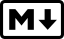
\includegraphics{figures/Markdown-mark.png} .

В настоящее время язык широко используется следующими сайтами и организациями:

\begin{itemize}
\tightlist
\item
  \href{http://github.com}{GitHub.com} - GitHub Flavored Markdown (GFM) - сайт с публичными и частными Git-репозиториями;
\item
  \href{https://bitbucket.org}{BitBucket.org} - сайт с публичными и частными Git- и Mercurial- репозиториями;
\item
  \href{https://about.gitlab.com/}{GitLab.com} - система упраления проектами с поддержкой Git-репозиториев;
\item
  \href{https://www.atlassian.com/software/jira}{Atlassian JIRA} - система управления задачами и проектами;
\item
  \href{https://wordpress.com/}{WordPress.com} - веб-платформа для создания сайтов и блогов;
\item
  \href{https://stackoverflow.com/}{StackOverflow.com} - сеть сайтов вопросов и ответов по множеству тематик.
\end{itemize}

Язык Markdown обладает следующими преимуществами:

\begin{itemize}
\tightlist
\item
  текстовый удобный для редактирования и чтения формат;
\item
  легко просматривать отличия между версиями и искать текст файловым менеджером и даже командой \texttt{grep};
\item
  возможна совместная работа в системе контроля версий (Git, Mercurial и пр.).
\end{itemize}

Для редактирования и просмотра Markdown документов может использоваться текстовый редактор с поддержкой Markdown:

\begin{itemize}
\tightlist
\item
  ReText (Windows, Linux - \url{https://github.com/retext-project/retext});
\item
  GhostWriter (Windows, Linux - \url{https://wereturtle.github.io/ghostwriter});
\item
  Typora (Windows, Linux, macOS - \url{https://typora.io/});
\item
  Remarkable (Windows, Linux - \url{http://remarkableapp.github.io/});
\item
  Geany (Windows, Linux, macOS - \url{https://geany.org/});
\item
  Atom text editor (Windows, Linux, macOS - \url{https://atom.io/});
\item
  Dilinger (online - \url{https://dillinger.io}).
\end{itemize}

Практически все редакторы имеют одинаковые стандартные возможности: форматирование, отображение Markdown и экспорт в HTML, PDF, ODT (OpenDocument) и др.

Настоящий документ написан с использованием обобщенного синтаксиса Markdown, поэтому изучение синтаксиса языка можно выполнять путем просмотра и/или редактирования отдельных элементов текста документа.

\section{Синтаксис Markdown}\label{markdown-syntax}

Далее рассматривается обобщенный Markdown синтаксис, включающий в себя:

\begin{itemize}
\tightlist
\item
  исходный \textbf{Makdown} синтаксис (см. \url{http://daringfireball.net/projects/markdown});
\item
  расширение \textbf{RMarkdown} (см. \href{https://raw.githubusercontent.com/rstudio/cheatsheets/master/rmarkdown-2.0.pdf}{RMarkdown Cheat Sheet} и \href{https://www.rstudio.com/wp-content/uploads/2015/03/rmarkdown-reference.pdf}{RMarkdown Reference});
\item
  \textbf{bookdown} для написания книг (см. \href{https://bookdown.org/yihui/bookdown/}{книгу Yihui Xie ``bookdown: Authoring Books and Technical Documents with R Markdown''}).
\end{itemize}

Исходный синтаксис \textbf{Markdown} обеспечивает форматирование документа.

\textbf{RMarkdown} позволяет выполнять расчеты на языке программирования R 
\includegraphics{figures/Rlogo.png} (см. \url{https://www.r-project.org/}) и оформлять полученные результаты в одном документе.

\textbf{Bookdown} -- это расширение RMarkdown для создания книг, его создал Yihui Xie в 2016 году. Официальная книга постоянно обновляется и расположена по адресу \url{https://bookdown.org/yihui/bookdown/}.

Назначение bookdown: автоматизированное получение из одного Rmd-документа файлов любых форматов (PDF, epub, HTML, docx, Mobi).

Дополнительная функциональность bookdown:

\begin{itemize}
\tightlist
\item
  Автоматическое создание оглавления.
\item
  Автоматическая одноуровневая или двухуровневая нумерация рисунков, таблиц, формул, теорем, доказательств и т.п.
\item
  Построение списка литературы в тексте учетом выбранного стиля оформления (например, в порядке упоминания источников).
\item
  Использование вычислительных возможностей языка R - возможность расчета графиков и вставки их в текст, включение файлов в текст.
\item
  Возможность выполнения программ скриптов в операционной системе и их включения в текст.
\item
  Автоматическое создание алфавитного указателя в LaTeX и PDF.
\end{itemize}

\textbf{Программное обеспечение и особенности}. Для работы с RMarkdown требуется установить среду разработки RStudio 
\includegraphics{figures/rstudio.png} и TeXLive для экспорта в LaTeX и PDF. Эти вопросы рассмотрены подробнее в разделе \ref{software}. При этом процесс получения документов имеет вид:


\includegraphics{figures/Rmd.png}

Выходными форматами являются PDF, ODT, RTF, HTML, docx. Подробности этого процесса описаны в книгах Yihui Xie.

Перейдем к рассмотрению обобщенного синтаксиса Markdown.

\subsection{Заголовки}\label{markdown-syntax-head}

Заголовки в Markdown обозначаются с помощью символа ``решетка'' (\#). Заголовок 1-го уровня имеет один символ \#, заголовок 2-го уровня - ``\#\#'' и т.п.

Заголовки могут иметь идентификатор, он указывается в фигурных скобках, см. например заголовок этого пункта. Все идентификаторы не должны содержать подчеркиваний (``\_``), но могут содержать знаки минус (''-``).

Ссылка на нумерованный раздел с известным идентификатором будет иметь вид: см. раздел \ref{markdown-syntax-head}.

Так же ссылка может быть задана с произвольным текстом: см. \hyperref[intro]{введение}. Этот вариант предпочтителен для экспорта в DOCX.

\subsection{Эффекты шрифта}\label{markdown-syntax-style}

Абзацы текста отделяется друг от друга переводами строки до и после.

Перевод текста на новую строку выполняется с помощью добавления двух пробелов\\
в конце строки (здесь три слова ``в конце строки'' оказались вначале новой строки).

Полужирный шрифт может быть получен одним из способов: \textbf{полужирный} или \textbf{полужирный}.

Курсивный шрифт может быть получен одним из способов: \emph{курсив} или \emph{курсив}.

Полужирный курсив может быть получен одним из способов: \textbf{\emph{полужирный курсив}} или \textbf{\emph{полужирный курсив}}.

После этого абзаца следует горизонтальная линия, заданная в виде трех последовательных знаков минус (``-''):

\begin{center}\rule{0.5\linewidth}{0.5pt}\end{center}

Моноширинный шрифт (обычно используется для отображения исходного кода) может быть задан с помощью двух символов машинописного обратного апострофа - \texttt{код\ в\ тексте}.

Многострочный исходный код отделяется от основного текста четырьмя пробелами:

\begin{verbatim}
int main() {
return 0;
}
\end{verbatim}

Цитаты или примечания оформляются с помощью знака больше (``\textgreater{}''):

\begin{quote}
Это цитата или примечание.
\end{quote}

Поскольку настоящий документ компилируется в RStudio, поэтому здесь поддерживаются дополнительные возможности RMarkdown:

\begin{itemize}
\tightlist
\item
  верхний индекс, например для возведения в квадрат - x\textsuperscript{2} ;
\item
  нижний индекс для индексации элементов - y\textsubscript{3} ;
\item
  зачеркнутых текст с помощью двойного знака тильды (``\textasciitilde{}'') : \st{зачеркнутый текст} ;
\item
  знак тире (``--'') в виде двух последовательных знаков минус : понятие -- опеределение ;
\item
  знак длинного тире (``---'') в виде трех последовательных знаков минус : понятие --- понятие .
\end{itemize}

\subsection{Списки}\label{markdown-syntax-lists}

Ниже представлен нумерованный список из трех пунктов (нумерация выполняется автоматически)

\begin{enumerate}
\def\labelenumi{\arabic{enumi}.}
\tightlist
\item
  Первый элемент списка;
\item
  Второй элемент списка;
\item
  Третий элемент списка.
\end{enumerate}

\begin{quote}
Примечание: автоматическая нумерация вложенных списков не поддерживается.
\end{quote}

Ниже представлен ненумерованный список из трех элементов

\begin{itemize}
\tightlist
\item
  Верхний элемент списка;
\item
  Средний элемент списка;
\item
  Нижний элемент списка.
\end{itemize}

Списки могут быть вложенными, при этом уровни отделяются двумя пробелами:

\begin{itemize}
\tightlist
\item
  1-й элемент уровня 1
\item
  2-й элемент уровня 1

  \begin{itemize}
  \tightlist
  \item
    1-й элемент уровня 2

    \begin{itemize}
    \tightlist
    \item
      1-й элемент уровня 3
    \end{itemize}
  \end{itemize}
\end{itemize}

Элементы списка могут содержать форматирование (полужирный шрифт, курсив, моноширинный шрифт и т.п.), могут содержать вложенные элементы. При этом код должен быть отделен необходимым дополнительным количеством пробелов:

\begin{itemize}
\item
  строка 1
\item
  строка 2 с блоком кода

\begin{verbatim}
int main(){
  return 0;
}
\end{verbatim}

  Далее следует цитата

  \begin{quote}
  Цитата
  \end{quote}

  и нумерованный список

  \begin{enumerate}
  \def\labelenumi{\arabic{enumi}.}
  \tightlist
  \item
    один
  \item
    два
  \item
    три
  \end{enumerate}
\item
  строка 3
\end{itemize}

\subsection{Ссылки и сноски}\label{markdown-syntax-links}

Ниже представлена \textbf{ссылка} на сайт университета:

\href{http://www.mpei.ru}{Сайт НИУ ``МЭИ''}

В квадратных скобках указан текст ссылки, который будет отображаться на экране, а в круглых скобках указывается полный URL ресурса.

В этом абзаце имеется \textbf{сноска} \footnote{Текст сноски} с расшифровкой в конце страницы.

\subsection{Изображения}\label{markdown-syntax-media}

Простой Markdown не позволяет выполнять автоматическую нумерацию рисунков, но позволяет вставить \textbf{рисунок} c подписью. Далее следует рисунок с названием \emph{Markdown}, сохраненный в файле \textbf{figures/Markdown-mark.png}:

\begin{figure}
\centering
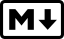
\includegraphics{figures/Markdown-mark.png}
\caption{Markdown}
\end{figure}

Рисунок может не иметь названия, тогда код упрощается:

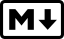
\includegraphics{figures/Markdown-mark.png}

Автоматическая нумерация рисунков выполняется с помощью метки \texttt{fig}, поэтому рисунок с автоматической нумерацией и идентификатором \texttt{md-logo} может быть вставлен следующим образом:

\begin{figure}
\centering
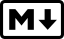
\includegraphics{figures/Markdown-mark.png}
\caption{\label{fig:md-logo} Логотип Markdown}
\end{figure}

Ссылка на такой рисунок будет иметь вид: на рисунке \ref{fig:md-logo} представлен логотип языка разметки Markdown.

Текст, обозначающий иллюстрацию (например, ``Рис.'' или ``Рисунок'') задается в файле \texttt{\_bookdown.yml} в YAML-секции \texttt{language}:

\begin{verbatim}
language:
  label:
    fig: 'Рисунок '
\end{verbatim}

Для каждого рисунка могут быть принудительно заданы его размеры с помощью соответствующих атрибутов \texttt{width} или \texttt{height} внутри фигурных скобок после описания изображения. Поддерживаются следующие единицы измерения \texttt{px}, \texttt{cm}, \texttt{mm}, \texttt{in} / \texttt{inch} и \texttt{\%}. Для сохранения пропорций рекомендуется задавать один размер (ширину или высоту).

Пример задания ширины изображения:

\begin{figure}
\centering
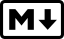
\includegraphics[width=1cm,height=\textheight]{figures/Markdown-mark.png}
\caption{\label{fig:md-logo-w-1cm} Логотип Markdown шириной 1 см}
\end{figure}

Пример задания высоты изображения:

\begin{figure}
\centering
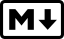
\includegraphics[width=\textwidth,height=2cm]{figures/Markdown-mark.png}
\caption{\label{fig:md-logo-h-2cm} Логотип Markdown высотой 2 см}
\end{figure}

Пример задания ширины и высоты изображения:

\begin{figure}
\centering
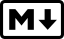
\includegraphics[width=\textwidth,height=39mm]{figures/Markdown-mark.png}
\caption{\label{fig:md-logo-w-64mm-h-39mm} Логотип Markdown шириной 64 мм и высотой 39 мм}
\end{figure}

\subsection{Таблицы}\label{markdown-syntax-tables}

Таблицы могут оформляться одним из способов - первый:

\begin{longtable}[]{@{}ll@{}}
\toprule\noalign{}
\textbf{Столбец 1} & \textbf{Столбец 2} \\
\midrule\noalign{}
\endhead
\bottomrule\noalign{}
\endlastfoot
строка 1, столбец 1 & строка 1, столбец 2 \\
строка 2, столбец 1 & строка 2, столбец 2 \\
\end{longtable}

второй:

\begin{longtable}[]{@{}ll@{}}
\toprule\noalign{}
\textbf{Столбец 1} & \textbf{Столбец 2} \\
\midrule\noalign{}
\endhead
\bottomrule\noalign{}
\endlastfoot
строка 1, столбец 1 & строка 1, столбец 2 \\
строка 2, столбец 1 & строка 2, столбец 2 \\
\end{longtable}

Выравнивание столбцов выполняется с помощью знака двоеточия (``:'') во второй строке:

\begin{longtable}[]{@{}
  >{\raggedright\arraybackslash}p{(\columnwidth - 4\tabcolsep) * \real{0.3247}}
  >{\centering\arraybackslash}p{(\columnwidth - 4\tabcolsep) * \real{0.3506}}
  >{\raggedleft\arraybackslash}p{(\columnwidth - 4\tabcolsep) * \real{0.3247}}@{}}
\toprule\noalign{}
\begin{minipage}[b]{\linewidth}\raggedright
\textbf{Столбец 1 (влево)}
\end{minipage} & \begin{minipage}[b]{\linewidth}\centering
\textbf{Столбец 2 (по центру)}
\end{minipage} & \begin{minipage}[b]{\linewidth}\raggedleft
\textbf{Столбец 3 (вправо)}
\end{minipage} \\
\midrule\noalign{}
\endhead
\bottomrule\noalign{}
\endlastfoot
строка 1, столбец 1 & строка 1, столбец 2 & строка 1, столбец 3 \\
строка 2, столбец 1 & строка 2, столбец 2 & строка 2, столбец 3 \\
\end{longtable}

Автоматическая нумерация таблиц выполняется с помощью метки \texttt{tab} аналогично рисункам.

\begin{longtable}[]{@{}ll@{}}
\caption{\label{tab:uno-tech} Технические характеристики платы Arduino Uno R3}\tabularnewline
\toprule\noalign{}
\textbf{Параметр} & \textbf{Значение} \\
\midrule\noalign{}
\endfirsthead
\toprule\noalign{}
\textbf{Параметр} & \textbf{Значение} \\
\midrule\noalign{}
\endhead
\bottomrule\noalign{}
\endlastfoot
Микроконтроллер & ATmega328P \\
Напряжение питания & 5 В \\
Внешнее напряжение питания (рекомендуемое) & 7--12 В \\
Внешнее напряжение питания (предельное) & 6--20 В \\
\end{longtable}

\begin{quote}
Примечание: английская надпись ``Table:'' обязательно должна присутствовать в начале строки для правильной нумерации таблицы.
\end{quote}

Ссылка на таблицу выполняется аналогично рисунку: в таблице \ref{tab:uno-tech} представлены технические характеристики платформы Arduino Uno.

Текст, обозначающий таблицу (например, ``Табл.'' или ``Таблица'') задается в файле \texttt{\_bookdown.yml} в YAML-секции \texttt{language}:

\begin{verbatim}
language:
  label:
    tab: 'Таблица '
\end{verbatim}

Текст в таблицах может иметь форматирование.

В некоторых случаях требуется поместить несколько строк текста в одну ячейку таблицы. При этом используется другой способ задания таблиц, который показан ниже при оформлении таблицы \ref{tab:soft-math-tab}.

\begin{longtable}[]{@{}
  >{\raggedleft\arraybackslash}p{(\columnwidth - 4\tabcolsep) * \real{0.0929}}
  >{\raggedright\arraybackslash}p{(\columnwidth - 4\tabcolsep) * \real{0.3388}}
  >{\raggedright\arraybackslash}p{(\columnwidth - 4\tabcolsep) * \real{0.5628}}@{}}
\caption{\label{tab:soft-math-tab} Программы и языки программирования для математических расчетов}\tabularnewline
\toprule\noalign{}
\begin{minipage}[b]{\linewidth}\raggedleft
\end{minipage} & \begin{minipage}[b]{\linewidth}\raggedright
\textbf{Визуальные}
\end{minipage} & \begin{minipage}[b]{\linewidth}\raggedright
\textbf{Текстовые}
\end{minipage} \\
\midrule\noalign{}
\endfirsthead
\toprule\noalign{}
\begin{minipage}[b]{\linewidth}\raggedleft
\end{minipage} & \begin{minipage}[b]{\linewidth}\raggedright
\textbf{Визуальные}
\end{minipage} & \begin{minipage}[b]{\linewidth}\raggedright
\textbf{Текстовые}
\end{minipage} \\
\midrule\noalign{}
\endhead
\bottomrule\noalign{}
\endlastfoot
\textbf{Платные} & \begin{minipage}[t]{\linewidth}\raggedright
\begin{itemize}
\tightlist
\item
  \href{http://www.ptc.com/product/mathcad}{PTC MathCAD}
\item
  \href{http://www.wolfram.com/mathematica}{Wolfram Mathematica}
\item
  \href{http://www.maplesoft.com}{Waterloo Maple}
\end{itemize}
\end{minipage} & \begin{minipage}[t]{\linewidth}\raggedright
\begin{itemize}
\tightlist
\item
  \href{http://www.mathworks.com}{MathWorks MATLAB}
\end{itemize}
\end{minipage} \\
\textbf{Бесплатные} & \begin{minipage}[t]{\linewidth}\raggedright
\begin{itemize}
\tightlist
\item
  \href{http://smath.info}{SMath Studio}
\item
  \href{http://www.wolframalpha.com}{WolframAlpha}
\item
  \href{http://andrejv.github.io/wxmaxima}{wxMaxima}
\end{itemize}
\end{minipage} & \begin{minipage}[t]{\linewidth}\raggedright
\begin{itemize}
\tightlist
\item
  \href{http://scilab.org/}{Scilab}
\item
  \href{https://www.gnu.org/software/octave/}{GNU Octave}
\item
  \href{http://www.sagemath.org/}{Sage}
\item
  \href{http://freemat.sourceforge.net/}{FreeMAT}
\item
  \href{http://axiom-developer.org}{Axiom}
\item
  \href{https://reduce-algebra.sourceforge.io}{Reduce}
\item
  \href{http://euler.rene-grothmann.de/index.html}{Euler Math Toolbox}
\item
  \href{http://julialang.org/}{Julia}
\item
  \href{https://code.google.com/p/spyderlib/}{Spyder - The Scientific PYthon Development EnviRonment}
\item
  \href{https://cran.rstudio.com/}{R}, \href{https://rstudio.com/products/rstudio/}{RStudio}
\item
  написание программ на языках \href{http://en.wikipedia.org/wiki/Fortran}{Fortran},
  \href{http://en.wikipedia.org/wiki/C_(programming_language)}{C}/\href{http://en.wikipedia.org/wiki/C++}{C++} с
  библиотеками \href{http://www.netlib.org/lapack/}{LAPACK}, \href{http://www.netlib.org/blas/}{BLAS},
  \href{http://math-atlas.sourceforge.net/}{ATLAS},
  \href{http://www.netlib.org/minpack/}{MINPACK}, \href{http://netlib.org/}{NETLIB.org},
  \href{http://arma.sourceforge.net/}{Armadillo}
\end{itemize}
\end{minipage} \\
\end{longtable}

\begin{quote}
Примечание: еще большее количество типов таблиц можно найти внутри документа \href{https://gitlab.iaaras.ru/iaaras/gostdown/blob/master/demo-main.md}{проекта GostDown} или в \href{https://pandoc.org/MANUAL.html\#tables}{соответствующем разделе документации по Pandoc}.
\end{quote}

\subsection{Формулы}\label{markdown-syntax-math}

Формулы без нумерации и расположенные непосредственно могут быть набраны в одиночных знаках доллара, например, \(a^2 + b^2 = c^2\).

Формулы без нумерации и расположенные в отдельной строке могут быть набраны в двойных знаках доллара в отдельной строке, как показано ниже

\[ E = \frac{mc^2}{\sqrt{1-\frac{v^2}{c^2}}} \]

или

\[
E = \frac{mc^2}{\sqrt{1-\frac{v^2}{c^2}}}
\]

Формулы с автоматической нумерацией отличаются наличием идентификатора в круглых скобках \texttt{(\textbackslash{}\#eq:name)}:

\begin{equation}
f\left(k\right) =\binom{n}{k} p^k\left(1-p\right)^{n k}
\label{eq:binom}
\end{equation}

При необходимости формула и ее номер могут быть правильно выравнены в MS Word с помощью применения пользовательского стиля \emph{DisplayEquation}:

\begin{equation}
S_{AM}\left( t \right) = U\left( 1+M\cdot F\left( t \right) \right)\cos \left( \omega_c\cdot t \right)
\label{eq:am}
\end{equation}

Ссылка на формулу выполняется с помощью поля \texttt{\textbackslash{}@ref(eq:name)}: ссылаемся на первое выражение - \eqref{eq:binom} и второе выражение \eqref{eq:am}.

Набор формул возможен в MathType 6 (желательно 6.9 и выше) с последующим экспортом в LaTeX с помощью меню \emph{Preferences} - \emph{Cut and Copy Preferences} : в списке \emph{MathML or TeX} нужно выбрать пункт \emph{Plain TeX}.

Для быстроты копирования можно снять обе галочки: \emph{Include translator name in translation} и \emph{Include MathType data in translation}.\\
Но иногда при экспорте в docx возникают ошибки pandoc вида \texttt{{[}pandoc\ warning{]}\ Cannot\ convert\ the\ following\ TeX\ math,\ skipping:}, поэтому лучше использовать LyX для набора или исправления формул.

\subsubsection{Формулы с матрицами}\label{markdown-syntax-math-matrix}

Матрицы:

\[AA = \begin{pmatrix} \alpha_{22} & \beta\\
 \Xi^2 & 1
\end{pmatrix}\]

\[\begin{pmatrix} 1 & 2 \\ 3 & 4 \end{pmatrix},
\begin{bmatrix} 1 & 2 \\ 3 & 4 \end{bmatrix},
\begin{vmatrix} 1 & 2 \\ 3 & 4 \end{vmatrix},
\begin{Vmatrix} 1 & 2 \\ 3 & 4 \end{Vmatrix}\]

Матрица с точками:

\[A = \begin{pmatrix}
a_{11} & a_{12} & \cdots & a_{1n} \\
a_{21} & a_{22} & \cdots & a_{2n} \\
\vdots & \vdots & \ddots & \vdots \\
a_{n1} & a_{n2} & \cdots & a_{nn}
\end{pmatrix}\]

Система уравнений со скобкой:

\begin{equation*}
 \begin{cases}
   2 |x|(2 - x) = a, \\
   x < 2, \\
   x \ne 0.
 \end{cases}
\end{equation*}

\subsubsection{Формулы с интегралами и дифференциалами}\label{markdown-syntax-math-syms}

В этом разделе собраны символы, наиболее часто используемые в дифференциальном и интегральном исчислении:

\begin{itemize}
\tightlist
\item
  \texttt{lim} предел;
\item
  \texttt{prod} произведение;
\item
  \texttt{sum} сумма;
\item
  \texttt{frac} черта деления;
\item
  \texttt{int} интеграл;
\item
  \texttt{iint} двойной интеграл;
\item
  \texttt{iiint} тройной интеграл;
\item
  \texttt{oint} круговой интеграл;
\item
  \texttt{partial} частная производная;
\item
  \texttt{infty} бесконечность;
\item
  \texttt{to} стрелка (в пределах);
\item
  \texttt{pm} плюс-минус
\end{itemize}

Дроби, в которых числитель расположен над знаменателем, набираются с помощью команды \(\frac{числитель}{знаменатель}\).

Производная в виде дроби:

\begin{equation}
F(x) = 2+\frac{d}{dx}(U(x))
\end{equation}

Частная производная:

\begin{equation}
dz = \frac{\partial z}{\partial x} dx + \frac{\partial z}{\partial y} dy
\end{equation}

Интегралы:

\begin{equation}
\int_{0}^{3} f(x) dx
\end{equation}

\begin{equation}
\iint_{x^2 + y^2 = 1} f(x, y) dx dy
\end{equation}

\begin{equation}
\iiint_{x^2 + y^2 + z^2 = 1} f(x, y, z) dx dy dz
\end{equation}

Пределы:

\begin{equation}
\lim\limits_{x \to \infty} \left(1 + \frac{1}{n} \right)^n = e
\end{equation}

Произведение:

\begin{equation}
F(x)= \prod_{n=1}^{\infty}\left(1 + \frac{x}{n!} \right)
\end{equation}

Функции:

\begin{equation}
    \lim_{n \to \infty}
    \sum_{k=1}^n \frac{1}{k^2}
    = \frac{\pi^2}{6}
\end{equation}

\begin{equation}
\arg, \cos, \cosh, \cot, \coth, \csc,\det, \dim, \exp, \gcd, \hom, \inf, \ker, \lg, \ln
\end{equation}

\begin{equation}
\log, \max, \min, \sec, \sin, \sinh, \sup,\tan, \tanh, \arccos, \arcsin, \arctan
\end{equation}

\begin{equation}
    \begin{matrix}
    \hat{\Phi}[k,l] & =
    & \left\{
    \begin{matrix}
    0 & \mbox{if } k,l = 0 \\
    S_x[k,l]\cdot H_x[k,l] + S_y[k,l]\cdot H_y[k,l] & \mbox{otherwise }
    \end{matrix} \right.
    \end{matrix}
\end{equation}

\begin{equation}
S_{\text{вых}}(x_2, y_2) = A_0 \underbrace{\iint dx_0 dy_0 \; g(x_0, y_0) \cdot h(x_2-x_0, y_2 -y_0)}_{\text{по определению это есть свёртка }} = A_0 g \otimes h
\end{equation}

\subsubsection{Примеры формул}\label{markdown-syntax-math-examples}

Амплитудная модуляция:

\begin{equation}
S_{AM}(t)=U(1+M \cdot F(t)) \cos{(\omega t+\phi)}
\end{equation}

Амплитудная однотональная модуляция:

\begin{equation}
S_{AM}(t)=U(1+M \cdot \cos{(\Omega t)}) \cos{(\omega_{c} t+\phi)}
\end{equation}

Амплитудная однотональная модуляция, разложение:

\begin{eqnarray}
S_{AM}(t)=U(1+M \cdot \cos{(\Omega t)}) \cos{( \omega_{c} t)} = \nonumber
\\
 = U \cos{(\omega t)} +U \cdot M \cdot \cos{(\Omega t)}) \cos{(\omega_{c} t)} =\nonumber
\\
 = U \cos{(\omega_{c} t)} +\frac{U \cdot M}{2} \cos{((\omega_{c}-\Omega) t)}) + \frac{U \cdot M}{2} \cos{((\omega_{c}+\Omega) t)})
\end{eqnarray}

\begin{eqnarray}
S_{AM}(t)= \underbrace{U \cos{(\omega_{c} t)}}_{\text{несущая}} +\nonumber
\\
+ \underbrace{\frac{U \cdot M}{2} \cos{((\omega_{c}-\Omega) t)})}_{\text{нижняя боковая полоса}} +\nonumber
\\
+\underbrace{\frac{U \cdot M}{2} \cos{((\omega_{c}-\Omega) t)})}_{\text{верхняя боковая полоса}} \nonumber
\end{eqnarray}

Частотная модуляция:

\begin{equation}
S_{FM}(t)=U \cos{((\omega_{c}+D \cdot F(t)) t+\phi)}
\end{equation}

Фазовая модуляция:

\begin{equation}
S_{PM}(t)=U \cos{(\omega_{c} t+(\phi+D \cdot F(t)))}
\end{equation}

Коэффициент передачи ФНЧ:

\begin{equation}
K(\omega)= \frac {1}{1+j\omega \tau}
\end{equation}

Коэффициент передачи ФВЧ:

\begin{equation}
K(\omega)= \frac {j\omega \tau}{1+j\omega \tau}
\end{equation}

Последовательный колебательный контур:

\begin{equation}
K(\omega)= \frac{U_{C}}{E}= \frac { \frac{1}{j\omega C}}{j \omega L+ \frac{1}{j\omega C}+R}
\end{equation}

\begin{equation}
K(\omega)=  \frac {1}{1 -\omega^2 LC+j \omega RC}
\end{equation}

Формула с прямым русским (кириллическим) текстом:

\begin{equation}
U_\text{вых.} = U_\text{м} \cos(\omega t)
\end{equation}

Формула с курсивным русским (кириллическим) текстом:

\begin{equation}
U_\textit{вых.} = U_\textit{м} \cos(\omega t)
\end{equation}

\subsection{Список литературы и библиографические ссылки}\label{markdown-syntax-bib}

Список литературы задается в виде отдельного файла с записями в формате BibTeX (\emph{.bib}). Пример фрагмента файла \emph{bibliography.bib}:

\begin{verbatim}
@online{arduino,
  title = {Arduino – Home},
  url = {https://www.arduino.cc/},
}

@book{banzi,
  title = {Arduino для начинающих волшебников},
  publisher = {М.: Рид Групп},
  author = {{Массимо Банци}},
  year = {2012},
}
\end{verbatim}

Описание библиографической записи в формате BibTeX для книг может быть получено с сайта \href{https://books.google.ru/}{Google Books} - нужно найти книгу с помощью поиска, найти ссылку \emph{About this book} и перейти по ней, далее на открывшейся странице с описанием книги найти в области \emph{Export Citation} кнопку \emph{BiBTeX} и скопировать описание книги в bib-файл.

Каждый элемент bib-файла характеризуется типом (в этом примере это \texttt{@online} для веб-страницы и \texttt{@book} для книги) и идентификатором, следующим после открывающей фигурной скобки (в этом примере \texttt{arduino} и \texttt{banzi}).

Ссылка в тексте дается в квадратных скобках с указанием идентификатора объекта после символа @.

Пример ссылки в тексте: для изучения платформы Arduino см. веб-страницу проекта Arduino {[}\citeproc{ref-arduino}{1}{]} и книгу М. Банци {[}\citeproc{ref-banzi}{2}{]}.

При необходимости можно добавить ссылку с учетом номеров страниц: см. книгу М. Банци {[}\citeproc{ref-banzi}{2, с. 11}{]} или {[}\citeproc{ref-banzi}{2, с. 15--20}{]}.

Оформление списков литературы выполняется в соответствии с правилами, заданными в CSL-файле стиля ссылок в YAML-преамбуле. К этому документу подключен файл \emph{gost-r-7-0-5-2008-numeric.csl}, соответствующий ГОСТ Р 7.0.5-2008 с цифровой нумерацией источников в порядке их упоминания в тексте.

\subsection{Листинги исходного кода}\label{markdown-listings}

В некоторых случаях оказывается необходимым выполнять нумерацию фрагментов исходного кода (листингов). Для этого в файле \texttt{\_bookdown.yml} в секции \emph{language} можно переобозначить индекс, предназначенный для оформления примеров:

\begin{verbatim}
language:
  label:
    exm: 'Листинг '
\end{verbatim}

В этом случае фрагмент программы может быть оформлен с использованием пользовательского стиля \emph{ListingCaption} для docx следующим образом:

\begin{example}
\protect\hypertarget{exm:code-blink}{}\label{exm:code-blink}Программа для отображения работы программы с помощью светодиода
\end{example}

\begin{verbatim}
// зададим номер контакта, к которому подключен светодиод
int ledPin = 13;

// функция setup выполняется однократно при нажатии клавиши сброса или включении платы
void setup() {
  // инициализация контакта, к которому подключен светодиод как выходного (OUTPUT)
  pinMode(ledPin, OUTPUT);
}

// функция loop выполняется в бесконечном цикле
void loop() {
  digitalWrite(ledPin, HIGH);   // включаем светодиод (HIGH – это напряжение 5 В)
  delay(1000);                       // пауза 1000 мс
  digitalWrite(ledPin, LOW);    // выключаем светодиод (в этом случае LOW – это напряжение 0 В)
  delay(1000);                       // пауза 1000 мс
}
\end{verbatim}

Ссылка на листинг исходного кода оформляется в виде: см. листинг \ref{exm:code-blink}.

\subsection{Оглавление}\label{markdown-toc}

Оглавление или содержание задается в YAML-преамбуле документа и имеет вид:

\begin{verbatim}
---
toc-title: "Оглавление"
output:
  bookdown::word_document2:
    toc: true
    toc_depth: 5
  bookdown::html_document2:
    toc: true
    toc_depth: 5
---
\end{verbatim}

здесь \texttt{toc-title} задает текст, выводимый перед оглавлением, \texttt{toc:\ true} включает отображение оглавления, \texttt{toc\_depth} задает количество отображаемых уровней заголовков в оглавлении.

\subsection{Вычисления RMarkdown}\label{markdown-rmarkdown}

RMarkdown позволяет объединять в одном документе расчеты и оформление результатов. Ниже представлен код для создания вложенного нумерованного списка:

\begin{enumerate}
\def\labelenumi{\arabic{enumi}.}
\tightlist
\item
  Пункт\\
  1.1. Подпункт\\
  1.2. Подпункт\\
\item
  Пункт
\end{enumerate}

\section{Необходимое программное обеспечение}\label{software}

Для локальной работы необходимо установить следующие компоненты: язык программировани R, среду RStudio, и набор типографских программ TeXLive для подготовки LaTeX- и PDF-версий документа и редактор ReText для редактирования документов Markdown.

Для редактирования полученного docx-файла необходим Microsoft Office 2007 (с SP3 и со всеми обновлениями) или более новой версии.

Для работы с формулами внутри docx-файла необходим MathType версии 6.9 и выше.

\subsection{R, RStudio, TeXLive}\label{software-r}

\subsubsection{Установка под Windows}\label{software-r-windows}

Поддерживается 64-битная версия Windows 7 и выше. Процесс установки сводится к следующим шагам:

\begin{enumerate}
\def\labelenumi{\arabic{enumi}.}
\item
  Загрузить R 4.0.5 for Windows с \href{https://cran.r-project.org/bin/windows/base/old/4.0.5/R-4.0.5-win.exe}{официального сайта} и установить со всеми настройками по умолчанию.
\item
  Загрузить R for Windows Build Tools с \href{https://cran.r-project.org/bin/windows/Rtools/rtools40-x86_64.exe}{официального сайта} и установить со всеми настройками по умолчанию.
\item
  Загрузить редактор Notepad++ с \href{https://notepad-plus-plus.org/download/}{официального сайта} и установить со всеми настройками по умолчанию.
\item
  Для сборки демонстрационного примера потребуется загрузить Git for Windows с \href{https://git-scm.com/download/win}{официального сайта} и установить, выбрав на этапе \emph{Choosing the default editor used by Git} пункт \emph{Use Notepad++ as Git's default editor}.
\item
  Для удобства работы с Git-репозиториями рекомендуется дополнительно загрузить с \href{https://tortoisegit.org/download/}{официального сайта} и установить расширение TortoiseGit для Проводника.
\item
  Загрузить RStudio с \href{https://www.rstudio.com/products/rstudio/download/\#download}{официального сайта} и запустить установку файла \texttt{RStudio-....exe} и дождаться ее завершения.
\item
  Для сборки PDF-версии документа с помощью RStudio потребуется установить TeX-пакеты от проекта TeXLive.

  \begin{quote}
  \textbf{Примечание:} в сети попадаются инструкции по использованию под Windows дистрибутива \href{https://miktex.org/howto/install-miktex}{MikTeX}, но он не работает нормально совместно с RStudio.\\
  В дистрибутивах GNU/Linux применяется TeXLive, поэтому будем использовать именно его и под Windows.
  \end{quote}

  Установка TeXLive требует следующих действий:

  \begin{enumerate}
  \def\labelenumii{\arabic{enumii}.}
  \tightlist
  \item
    Загрузить дистрибутив TeXLive в виде ISO-файла \href{https://www.tug.org/texlive/acquire-iso.html\#torrent}{как торрент с официального сайта}.
  \item
    Подключить загруженный образ установочного диска в систему программой \href{https://www.osforensics.com/tools/mount-disk-images.html}{OSFMount} или аналогичной.
  \item
    Запустить установщик \texttt{install-tl-windows.bat}.
  \item
    В открывшемся окне нажать кнопку \emph{Установить}.
  \item
    По окончанию установки нажать кнопку \emph{Закрыть}.
  \end{enumerate}
\item
  Запустить RStudio и установить пакеты R для поддержки \href{https://bookdown.org/home/getting-started.html}{bookdown} через командную строку внутри RStudio, выполнив последовательно команду в окне \emph{Console}:

\begin{verbatim}
install.packages(c('markdown', 'bookdown', 'tikzDevice'), repos='http://cran.r-project.org')
\end{verbatim}

  и закрыть RStudio.
\item
  Для подготовки первого RMarkdown документа следует клонировать \href{https://github.com/k0ly4n/bookdown-demo-rus}{демонстрационный русифицированный репозиторий} с помощью Git - открыть Проводник, нажать правую кнопку мыши, выбрать в выпадающем меню пункт \emph{Git Bash Here}, вставить в командную строку команду

\begin{verbatim}
git clone https://github.com/k0ly4n/bookdown-demo-rus
\end{verbatim}

  нажать \texttt{\textless{}Enter\textgreater{}} и дождаться завершения клонирования, закрыть окно \emph{MINGW\ldots{}}.
\item
  Перейти в только что созданный каталог \texttt{bookdown-demo-rus} и выполнить двойной щелчок мышью по файлу \texttt{bookdown-demo-rus.Rproj} для открытия проекта книги в RStudio.
\item
  Дождаться открытия RStudio, выбрать в верхней правой части окна вкладку \emph{Build} и нажать стрелку вниз рядом с пунктом \emph{Build Book} и выбрать пункт \emph{bookdown:html\_document2} для подготовки HTML-версии книги.

  \begin{quote}
  \textbf{Примечание:} возможно появление окна \emph{Install Required Packages},
  в котором нужно нажать кнопку \emph{Yes} для установки пакетов.
  \end{quote}

  По завершению сборки откроется HTML-версия книги.

  \begin{quote}
  \textbf{Примечание:} если требуется подготовка книги в EPUB-формате (\emph{bookdown:epub\_book}), то для просмотра этого формата
  нужно установить дополнительный просмотрщик. Например, простой и легковесный \href{https://www.sumatrapdfreader.org/dl/rel/3.4.6/SumatraPDF-3.4.6-64-install.exe}{Sumatra PDF}.
  \end{quote}
\item
  Для сборки PDF-версии документа следует выбрать в верхней правой части окна RStudio вкладку \emph{Build} и нажать стрелку вниз рядом с пунктом \emph{Build Book} и выбрать пункт \emph{bookdown:pdf\_book}.
\end{enumerate}

\subsubsection{Установка под GNU/Linux}\label{software-r-linux}

В настоящее время существует два скрипта автоматизированной установки необходимого программного обеспечения:

\begin{enumerate}
\def\labelenumi{\arabic{enumi}.}
\tightlist
\item
  \href{https://github.com/N0rbert/umpis}{umpis} предназначен для систем на основе дистрибутива Debian, он поддерживает системы Debian (9, 10, 11 и 12), AstraLinux (2.12 и 1.7), Ubuntu MATE (18.04 LTS, 20.04 LTS и 22.04 LTS).
\item
  \href{https://github.com/N0rbert/alpis}{alpis} - для систем ALT Linux, созданных на основе 9-й и 10-й платформ (Workstation, MATE StarterKit и SimplyLinux).
\end{enumerate}

Многолетний опыт автора настоящего документа позволяет рекомендовать среду рабочего стола MATE для повседневного и повсеместного использования. В следующем подразделе приведены в том числе команды для установки среды MATE в систему Debian.

\paragraph{Установка под Debian}\label{software-r-linux-debian}

В системах Debian рекомендуется предварительно настроить использование команды \texttt{sudo} с помощью выполнения следующих команд, запущенных от имени пользователя \emph{root}:

\begin{verbatim}
apt-get update
apt-get install sudo
\end{verbatim}

и затем добавить пользователя в группу \emph{sudo} командой \texttt{su\ -l\ -c\ "usermod\ -a\ -G\ sudo\ \$USER"}, выполненной от обычного пользователя, и перезагрузить компьютер.

После этого среда MATE может быть установлена с помощью команды \texttt{sudo\ apt-get\ install\ task-mate-desktop\ mate-desktop-environment-extras}.

Для запуска скрипта \texttt{umpis.sh} в графической сессии MATE следует выполнить следующие команды в терминале:

\begin{verbatim}
sudo apt-get update
sudo apt-get install wget dconf-cli

cd ~/Downloads || cd ~/Загрузки
wget -c https://raw.githubusercontent.com/N0rbert/umpis/master/umpis.sh
chmod +x umpis.sh
sudo -E ./umpis.sh
\end{verbatim}

Большую часть времени скрипт работает автономно без участия пользователя. На финальном этапе скрипт задаст вопрос о выборе экрана входа в систему, на который нужно ответить выбором пункта \emph{sddm}; запросит у пользователя его пароль для установки среды программирования Arduino IDE и путь к каталогу ее установки. После окончания работы скрипта нужно перезагрузить компьютер, на экране входа выбрать сеанс MATE и авторизоваться.

\paragraph{Установка под ALT Linux}\label{software-r-linux-alt}

В системах ALT Linux Workstation и MATE StarterKit рекомендуется предварительно настроить использование команды \texttt{sudo} с помощью выполнения следующей команды, запущенной от обычного пользователя:

\begin{verbatim}
su -l -c "usermod -a -G wheel $USER; control sudo wheelonly; control sudoers relaxed; control sudoreplay wheelonly; control sudowheel enabled;"
\end{verbatim}

Для запуска скрипта \texttt{alpis.sh} в графической сессии MATE следует выполнить следующие команды в терминале:

\begin{verbatim}
sudo apt-get update
sudo apt-get install wget lsb-release

cd ~/Downloads || cd ~/Загрузки
wget -c https://raw.githubusercontent.com/N0rbert/alpis/master/alpis.sh
chmod +x alpis.sh
sudo -E ./alpis.sh
\end{verbatim}

Скрипт работает автономно. После окончания его работы нужно перезагрузить компьютер, на экране входа выбрать сеанс MATE и авторизоваться.

\subsection{Текстовый редактор ReText}\label{software-retext}

Редактирование отдельных Markdown файлов можно выполнять в простом визуальном редакторе \href{https://github.com/retext-project/retext}{ReText}. В зависимости от версии Windows его установка выполняется следующим образом:

\begin{itemize}
\tightlist
\item
  в Windows 7 нужно установить \href{https://www.python.org/ftp/python/3.8.10/python-3.8.10-amd64.exe}{Python 3.8.10} (поставив галочку \emph{Add Python 3.8 to PATH}) и затем установить ReText из репозитория PyPi с помощью команды \texttt{pip\ install\ ReText==7.2.3\ pyqtwebengine==5.15.2}.
\item
  в более новых версиях Windows нужно установить \href{https://www.python.org/downloads/windows/}{актуальную версию Python} и затем установить ReText из репозитория PyPi с помощью команды \texttt{pip\ install\ ReText\ pyqt6-webengine}.
\end{itemize}

После установки редактор ReText можно запустить командой \texttt{retext} и создать затем ярлык для программы.

\begin{quote}
\textbf{Примечание:} в случае если при открытии документа с русским текстом символы в редакторе отображаются некорректно, следует изменить шрифты на поддерживающие кириллицу.
Для этого следует нажать в меню \textbf{Edit} на пункт \textbf{Change editor font} для смены шрифта в редакторе и выбрать нужный шрифт (обычно моноширинный, например \emph{Courier New}).\\
Далее следует повторить действия для шрифта предварительного просмотра \textbf{Change preview font} и выбрать нужный шрифт (обычно не моноширинный, например \emph{Times New Roman}).
\end{quote}

В системах GNU/Linux редактор содержится в репозиториях под именем пакета \texttt{retext}. Для поддержки проверки орфографии нужно установить специальный пакет командой \texttt{sudo\ apt-get\ install\ python3-enchant} (Debian) или \texttt{sudo\ apt-get\ install\ python3-module-enchant} (ALT Linux).

Следует учитывать, что редактор ReText не поддерживает расширения RMarkdown. Однако, это не мешает их использованию и набору в тексте.

Для поддержки формул внутри текста (вида \texttt{\$...\$}) нужно включить в настройках расширение \texttt{mathjax} (в линуксе с помощью команды \texttt{echo\ mathjax\ \textgreater{}\ \$HOME/.config/markdown-extensions.txt}) и переключить режим предварительного просмотра на использование движка \emph{WebEngine (Chromium) Renderer} (или \emph{WebKit Renderer}) в меню \emph{Edit}.

Для игнорирования YAML заголовка нужно добавить в строку дополнений \texttt{meta}.

\section{Процесс подготовки odt-документов}\label{authoring-odt}

Для odt-документов требуются дополнительные действия.

\subsection{Использование odt-шаблона}\label{authoring-odt-template}

Для удовлетворения требований оформления под конкретный случай возможно создание и использование файла odt-шаблона. В этом файле задается формат страницы, поля страницы, стили заголовков и текста. Путь в файлу odt-шаблона задается в YAML-преамбуле:

\begin{verbatim}
---
output:
  bookdown::odt_document2:
    reference_docx: styles-reference.odt
---
\end{verbatim}

Файл шаблона может быть многократно последовательно изменен до получения качественного результата.

Особенности:

\begin{enumerate}
\def\labelenumi{\arabic{enumi}.}
\tightlist
\item
  На текущий момент не поддерживаются пользьзовательские стили оформления участков текста.
\item
  Формулы будут отображаться в формате OMML, их преобразование в MathType под GNU/Linux невозможно.
\end{enumerate}

\subsection{Финальная подготовка рукописи}\label{authoring-odt-final}

Финальная подготовка текста включает следующие этапы:

\begin{itemize}
\item
  оформление \textbf{страниц} и их порядок следования:

  \begin{enumerate}
  \def\labelenumi{\arabic{enumi}.}
  \tightlist
  \item
    Редактирование титульного листа в соответствии с требованиями.
  \item
    Перенос страницы задания и/или аннотации на второй лист (после титульного листа) перед оглавлением.
  \item
    Удаление нумерации перед следующими структурными элементами: \emph{Аннотация}, \emph{Введение}, \emph{Заключение}, \emph{Приложения}, \emph{Список использованных источников} (нужно нажать мышью на номер и выполнить удаление кнопкой \texttt{\textless{}Delete\textgreater{}}).
  \item
    Ручной перенос приложений в конец документа (после списка использованных источников).
  \item
    Ручное добавление заголовков ``Продолжение Приложения \#'' в случае если приложения состоят двух и более страниц.
  \end{enumerate}
\item
  оформление \textbf{таблиц}:

  \begin{enumerate}
  \def\labelenumi{\arabic{enumi}.}
  \tightlist
  \item
    Перенос названий и номеров таблиц снизу таблицы наверх.
  \item
    Ручное добавление текста ``Продолжение табл. \#'' в случае если таблица не помещается на одну страницу.
  \end{enumerate}
\item
  оформление \textbf{формул}:

  \begin{enumerate}
  \def\labelenumi{\arabic{enumi}.}
  \tightlist
  \item
    Выравнивание формулы и ее номера вручную с помощью соответствующего стиля.
  \end{enumerate}
\item
  действия \textbf{перед печатью}:

  \begin{enumerate}
  \def\labelenumi{\arabic{enumi}.}
  \tightlist
  \item
    Проверка правописания с корректировкой ошибок.
  \item
    Обновление всех ссылок документа с помощью последовательного нажатия комбинаций клавиш \texttt{\textless{}Ctrl+A\textgreater{}}, \texttt{\textless{}F9\textgreater{}} или из меню \emph{Tools → Update → Update All}.
  \end{enumerate}
\end{itemize}

\section{Процесс подготовки docx-документов}\label{authoring-docx}

Аналогично формату odt, для docx-документов требуются дополнительные действия.

\subsection{Использование docx-шаблона}\label{authoring-docx-template}

Для удовлетворения требований оформления под конкретный случай возможно создание и использование файла docx-шаблона. В этом файле задается формат страницы, поля страницы, стили заголовков и текста. Путь в файлу docx-шаблона задается в YAML-преамбуле:

\begin{verbatim}
---
output:
  bookdown::word_document2:
    reference_docx: styles-reference.docx
---
\end{verbatim}

Файл шаблона может быть многократно последовательно изменен до получения качественного результата.

\subsection{Преобразование формул}\label{authoring-docx-math}

RStudio использует Pandoc для преобразования документов из Markdown в другие форматы. Поэтому формулы оказываются преобразованными в формат OMML (Microsoft's Office Math Markup Language) вместо MathType. Но для издательства МЭИ и при оформлении дипломов и отчетов достаточно строго требуется использование MathType, поэтому необходимо выполнить конвертацию формул из OMML в MathType:

\begin{enumerate}
\def\labelenumi{\arabic{enumi}.}
\tightlist
\item
  Открыть docx-документ в Word (иногда \emph{Открыть и восстановить});
\item
  На ленте \emph{MathType} нажать кнопку \emph{Convert Equations};
  в открывшемся окне установить в области \emph{Equation types to convert} галочку \emph{Word 2007 and late (OMML) equations}, затем в области \emph{Convert equations to} выбрать \emph{MathType equations (OLE objects)}.
\item
  Нажать кнопку \emph{Convert} и ждать результата.
\item
  Отформатировать все формулы (греческие буквы - прямо и т.п.) - нажать на ленте \emph{MathType} кнопку \emph{Format Equations}, в области \emph{Format equations using preferences from} установить переключатель в положение \emph{MathType preference file}, нажать кнопку \emph{Browse}, выбрать файл настроек \texttt{format.eqp} и применить изменения кнопкой \emph{OK}.
\end{enumerate}

\textbf{Примечание:} При конвертации из OMML в MathType могут не работать LaTeX-окружения \texttt{split} и \texttt{multiline}, поэтому надежнее использовать \texttt{array}.

\subsection{Финальная подготовка рукописи}\label{authoring-docx-final}

Финальная подготовка текста включает следующие этапы:

\begin{itemize}
\item
  оформление \textbf{страниц} и их порядок следования:

  \begin{enumerate}
  \def\labelenumi{\arabic{enumi}.}
  \tightlist
  \item
    Выделение первой страницы под титульный лист и ее добавление в начало документа.
  \item
    Перенос страницы задания и/или аннотации на второй лист (после титульного листа) перед оглавлением.
  \item
    Удаление нумерации перед следующими структурными элементами: \emph{Аннотация}, \emph{Введение}, \emph{Заключение}, \emph{Приложения}, \emph{Список использованных источников} (нужно нажать мышью на номер и выполнить удаление кнопкой \texttt{\textless{}Delete\textgreater{}}).
  \item
    Ручной перенос приложений в конец документа (после списка использованных источников).
  \item
    Ручное добавление заголовков ``Продолжение Приложения \#'' в случае если приложения состоят двух и более страниц.
  \end{enumerate}
\item
  оформление \textbf{таблиц}:

  \begin{enumerate}
  \def\labelenumi{\arabic{enumi}.}
  \tightlist
  \item
    Ручное добавление текста ``Продолжение табл. \#'' в случае если таблица не помещается на одну страницу.
  \end{enumerate}
\item
  оформление \textbf{формул}:

  \begin{enumerate}
  \def\labelenumi{\arabic{enumi}.}
  \tightlist
  \item
    Преобразование всех формул из OMML в MathType (см. раздел \ref{authoring-docx-math} выше).
  \end{enumerate}
\item
  действия \textbf{перед печатью}:

  \begin{enumerate}
  \def\labelenumi{\arabic{enumi}.}
  \tightlist
  \item
    Проверка правописания с корректировкой ошибок.
  \item
    Обновление всех ссылок документа с помощью последовательного нажатия комбинаций клавиш \texttt{\textless{}Ctrl+A\textgreater{}}, \texttt{\textless{}F9\textgreater{}} и выбора пункта \emph{Обновить целиком} в диалоговом окне.
  \item
    Проверка отсутствия неработоспособных ссылок с помощью поиска (\texttt{\textless{}Ctrl+F\textgreater{}}, текст \emph{Ошибка!}).
  \end{enumerate}
\end{itemize}

\chapter{Вторая глава}\label{chapter2}

Это -- вторая глава

\chapter{Третья глава}\label{chapter3}

Это -- третья глава

\chapter*{Заключение}\label{conclusion}
\addcontentsline{toc}{chapter}{Заключение}

В заключении оратор сказал\ldots{}

\chapter*{Приложения}\label{appendix}
\addcontentsline{toc}{chapter}{Приложения}

Ну, это у кого не вырвали.\\
Мы про\ldots{} аппендицит, если что\ldots{}

\chapter*{Список использованных источников}\label{references}
\addcontentsline{toc}{chapter}{Список использованных источников}

В то числе и целебных\ldots{}

\phantomsection\label{refs}
\setlength{\cslhangindent}{0em}
\setlength{\cslentryspacing}{0em}
\begin{CSLReferences}
\bibitem[\citeproctext]{ref-arduino}
\CSLLeftMargin{1. }%
\CSLRightInline{Arduino -- Home {[}Электронный ресурс{]}. URL: \url{https://www.arduino.cc/}.}

\bibitem[\citeproctext]{ref-banzi}
\CSLLeftMargin{2. }%
\CSLRightInline{Массимо Банци. Arduino для начинающих волшебников. М.: Рид Групп, 2012.}

\end{CSLReferences}

\end{document}
